\section{Overview}
Here we represent an overview of how the entire BBP architecture is composed of:

\begin{figure}[htbp]
	\centering
	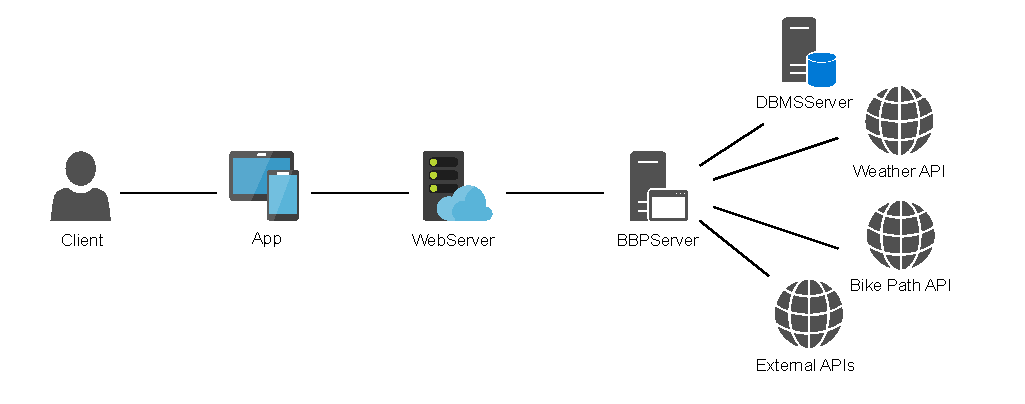
\includegraphics[width=\textwidth]{Images/Overview.drawio.pdf}
	\caption{Overview}
\end{figure}

\subsection{Client Side}
\begin{itemize}
	\item \textbf{Client}: Represents the end-user, categorized as either a Registered User or a Guest (Unregistered User). They interact with the platform to search for routes, record trips, or contribute road status data
	\item \textbf{App}: A mobile application, compatible with Android and iOS, that serves as the primary user interface. It is responsible for high-speed data acquisition from geospatial sensors (GPS) and Inertial Measurement Units (IMU) to track movement and detect road anomalies like potholes
\end{itemize}

\subsection{Server Side}
\begin{itemize}
	\item \textbf{API Gateway}: Acts as the secure entry point for all requests originating from the mobile application. It manages communication using HTTPS/TLS protocols to ensure the integrity of sensitive geolocation data transmitted to the backend. It is responsible for load balancing requests among BBP Server instance
	\item \textbf{BBP Server}: The central component of the system architecture that implements the core business logic. It handles Path Scoring and Ranking, resolves data conflicts during Information Merging, processes Automated Trip Recording guesses, and manages user authentication sessions
	\item \textbf{DBMS Server}: The Database Management System that serves as the persistent repository for the platform. It stores all data, including user profiles, saved routes, and system logs. It acts as the central repository for all essential information required by the platform
	\item \textbf{Weather API}: An interface with external meteorological services. It allows the system to retrieve real-time environmental data, like temperature and wind speed, to enrich trip logs with local weather context
	\item \textbf{Bike Path API}: A specialized external service utilized to Search Path. It provides the necessary data to visualize existing cycling networks
	\item \textbf{External APIs}: General category for third-party services. These are used for geocoding, street name resolution, and up-to-date base-map rendering to ensure the reliability of the road network presented to users, and most importantly to calculate the distance between points during recordings
\end{itemize}

\newpage
\section{Component View}
\subsection{High Level Diagram}

\begin{figure}[htbp]
	\centering
	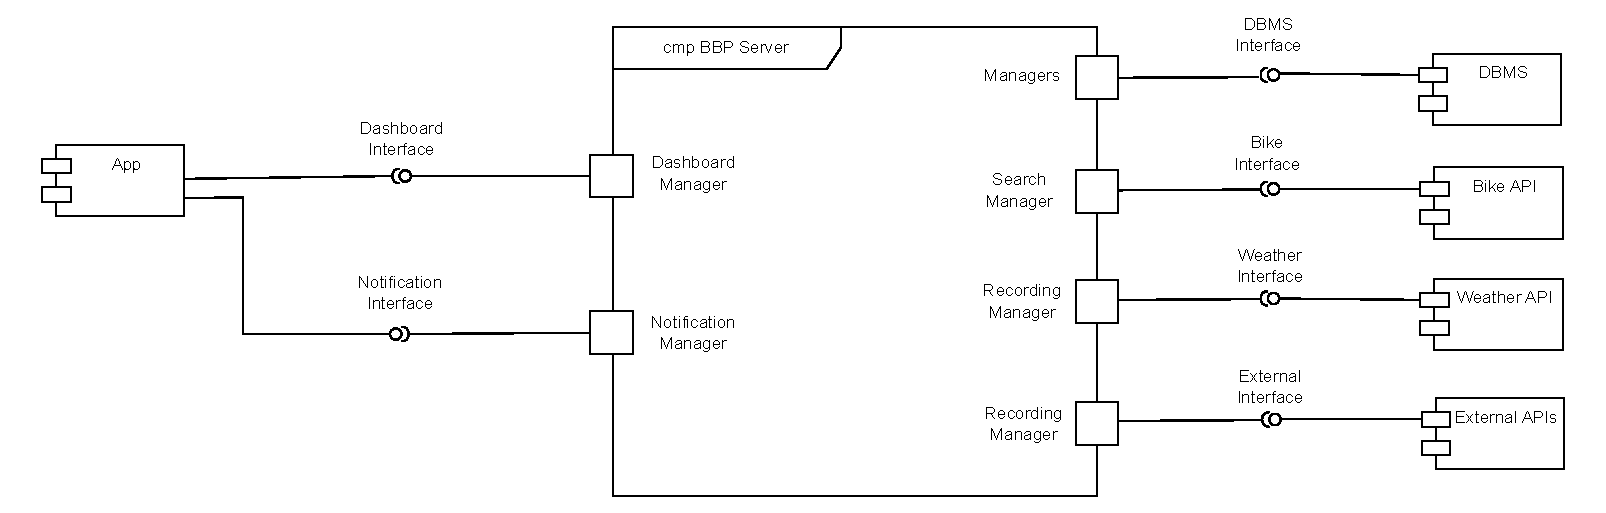
\includegraphics[width=\textwidth]{Images/HighLevel.drawio.pdf}
	\caption{High Level Diagram}
\end{figure}

In the figure above is the high-level component diagram of BBP where it's represented the external components 
of BBP and how they communicate with the BBP server, in particular:
\begin{itemize}
	\item \textbf{App}: This component represents the front-end interface used by cyclists to interact with the system. It communicates with the server via the Dashboard and Notification interfaces
	\item \textbf{DBMS (Database Management System)}: Connected via the DBMS Interface, this is the centralized repository for the system, it's used by different managers in the server application
	\item \textbf{Bike API}: The system communicates with this API to find cycling routes and retrieve up-to-date information regarding road networks and cycling-compatible paths, only used by search manager to respond request like search path in a zone
	\item \textbf{Weather API}: This dedicated service provides real-time meteorological conditions, such as temperature and wind speed, which the system uses to enrich trip data and help users analyze their performance relative to the environment. Only used by recording manager
	\item \textbf{External APIs}: These interfaces are used specifically for geocoding (converting coordinates to street names) and performing precise distance calculations between two GPS points. Only used by recording manager
\end{itemize}
\newpage

\subsection{Low Level Diagram}

\begin{figure}[htbp]
	\centering
	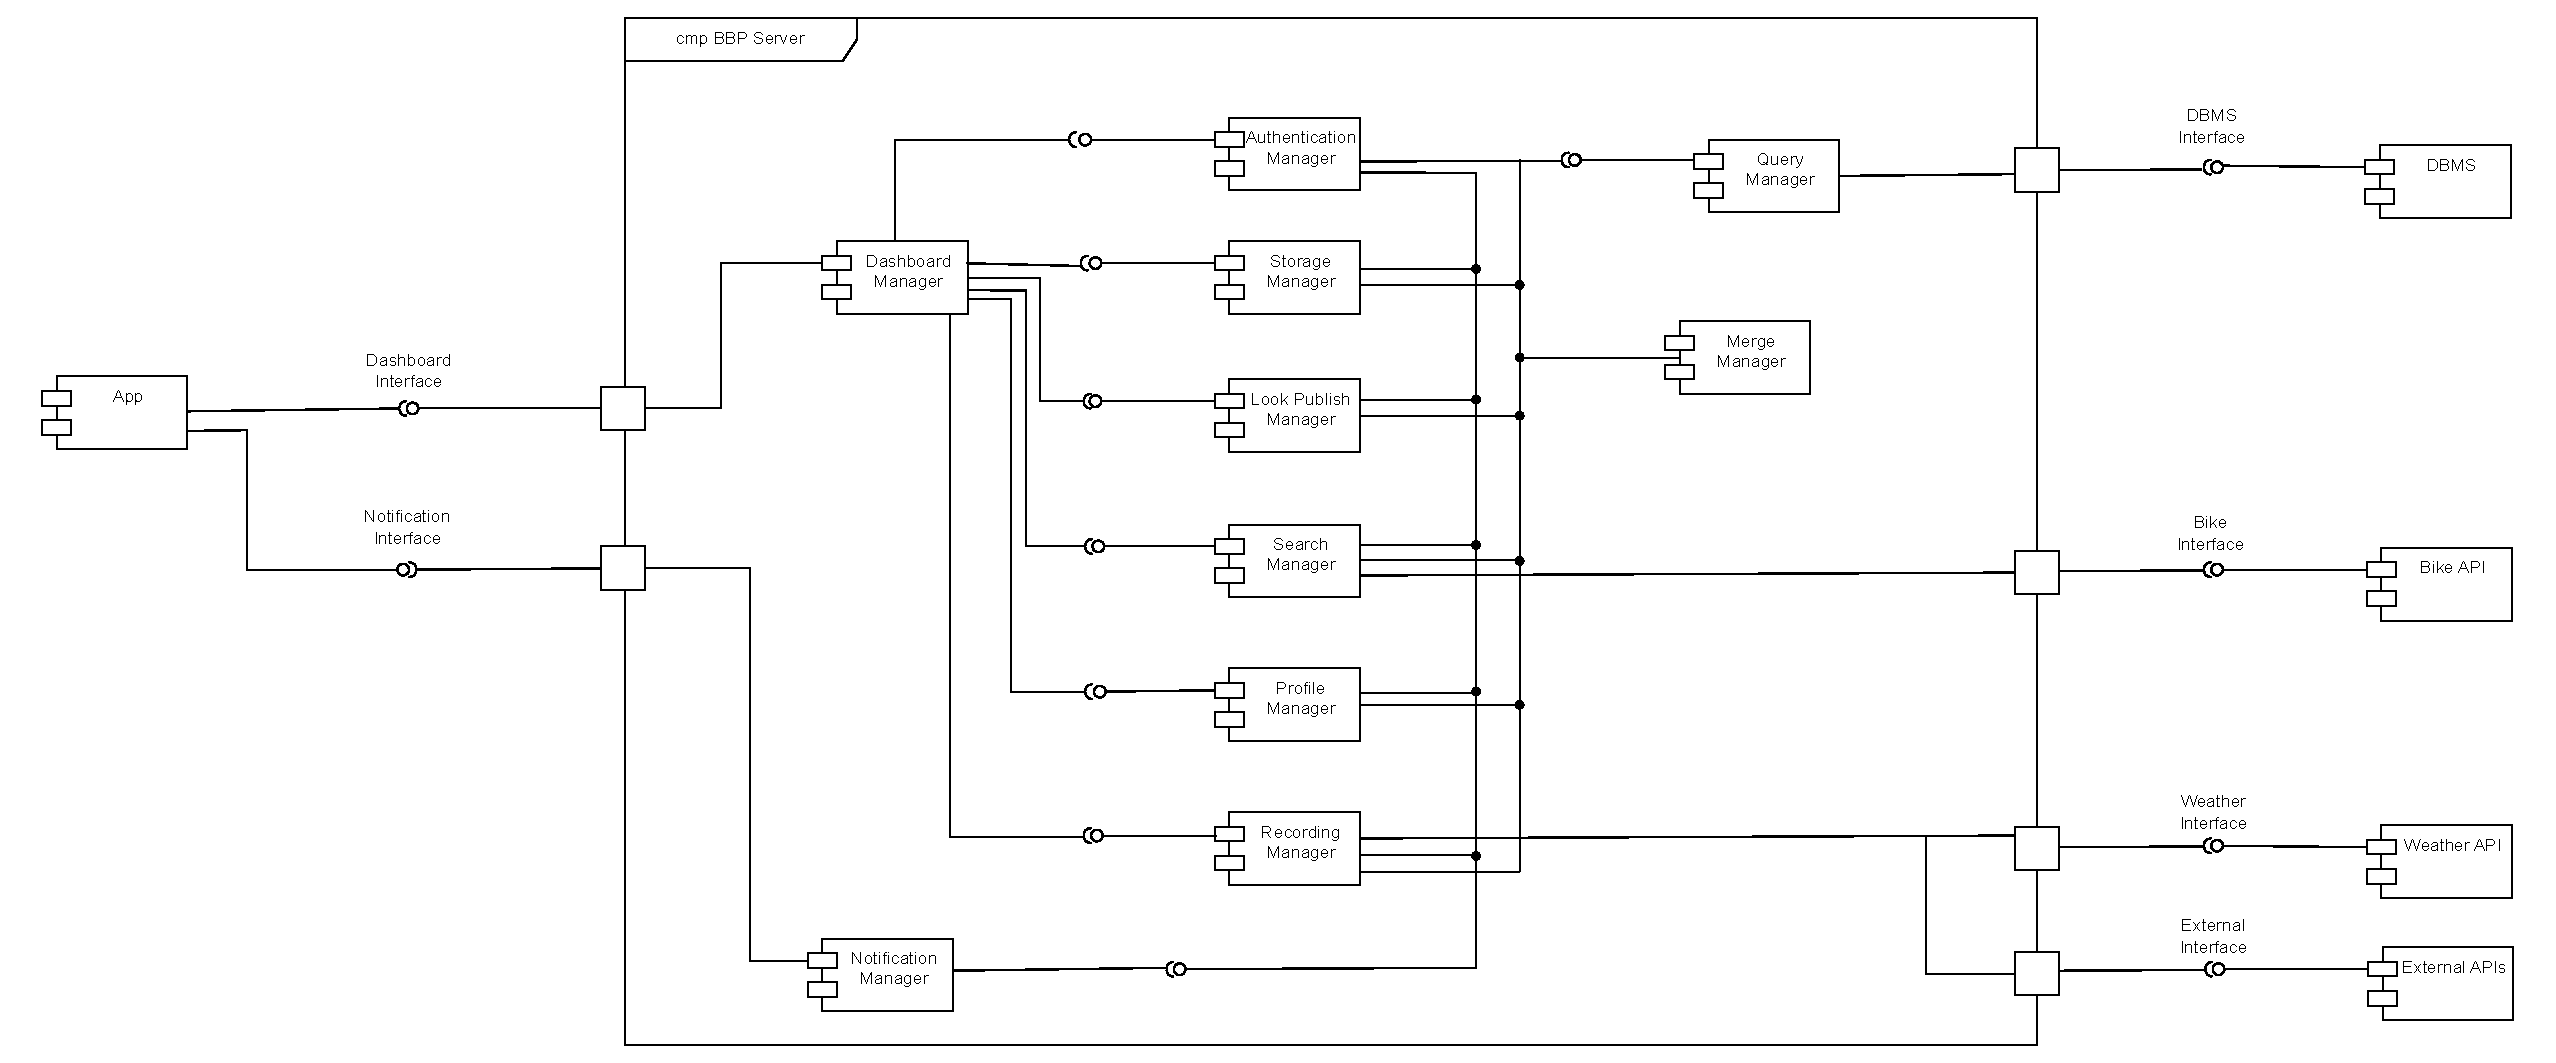
\includegraphics[width=\textwidth]{Images/LowLevel.drawio.pdf}
	\caption{Low Level Diagram}
\end{figure}

The figure above represents the complete architecture of BBP with each components inside the BBP Server:
\begin{itemize}
	\item \textbf{Authentication Manager}: Serves as the security gatekeeper for the BBP system. It is responsible for handling all procedures related to user identity verification, 
	including the registration of new accounts and the secure login of existing users. This component validates credentials against stored data, manages session states 
	(such as guest versus authenticated access), and ensures that only authorized users can access sensitive features like trip recording and history management
	\item \textbf{Dashboard Manager}: Acts as the central orchestration layer for the user interface, serving as the primary bridge between the mobile application (App) 
	and the various backend sub-systems. It aggregates data from the storage, profile, and recording modules to present a cohesive view to the user, such as displaying the "Home" screen 
	or summarizing recent activities. It ensures that the information requested by the Dashboard Interface is routed to the correct internal manager for processing
	\item \textbf{Storage Manager}: Is tasked with the persistence and retrieval of historical cycling data. It manages the user's personal log of completed trips, ensuring that GPS traces, 
	timestamped statistics (speed, distance), and performance metrics are securely saved for future reference. This component allows users to access their "Trip History" and is responsible 
	for differentiating between private data and data that has been flagged for public contribution
	\item \textbf{Look Publish Manager}: Facilitates the community-sharing aspects of the platform. It handles the logic required for browsing paths published by other users, 
	allowing the system to filter and retrieve "public" routes based on geographic areas. Furthermore, it manages the transition of a trip from a private recording to 
	a public resource, ensuring that the user's intent to share their route with the community is processed and reflected in the system
	\item \textbf{Search Manager}: Engineers the route discovery process. It processes user requests for paths between specific origin and destination points, calculating optimal 
	routes based on available data. This manager implements the scoring algorithms that evaluate paths not just by distance, but by the quality of the road surface and the absence of obstacles, 
	identifying the "best" path as defined by the community data
	\item \textbf{Profile Manager}: Administers all user-specific data and preferences. It allows registered users to view and update their personal details, 
	such as account credentials and privacy settings. Additionally, it aggregates cumulative statistics to provide the user with a comprehensive summary of their engagement with the platform
	\item \textbf{Recording Manager}: Orchestrates the active data acquisition lifecycle during a cycling session. It supports both "Manual Mode" (where users input data after a trip) and "Automated Mode" (which uses real-time GPS and sensor data). 
	It interfaces with external APIs and device sensors to capture geospatial coordinates and detect anomalies like potholes in real-time, preparing this raw data for validation and eventual storage
	\item \textbf{Notification Manager}: Handles the dissemination of system alerts and prompts to the user. It is responsible for triggering push notifications, such as the alert asking a user to confirm if they wish to start recording when cycling speed is detected. 
	It ensures that the user is prompted at the appropriate times to validate automated detections, such as confirming the presence of a pothole at the end of a trip
	\item \textbf{Merge Manager}: Implements the core logic for data consistency and conflict resolution. It is responsible for aggregating path information from multiple users regarding the same street segment. 
	This manager applies algorithms to weigh new data against historical records—prioritizing data freshness and confirmation counts, to update the global "score" and status of a path, ensuring the community map reflects the most accurate current conditions
	\item \textbf{Query Manager}: Serves as the data access layer, abstracting the complexity of the database interactions from the other business logic components. 
	It receives data requests from the various managers and translates them into operations compatible with the DBMS. It ensures that data is efficiently read from or written to 
	the underlying database infrastructure while maintaining data integrity
\end{itemize}

\subsubsection*{Recording Manager}
Here we describe the Recording Manager component in detail:

\begin{figure}[htbp]
	\centering
	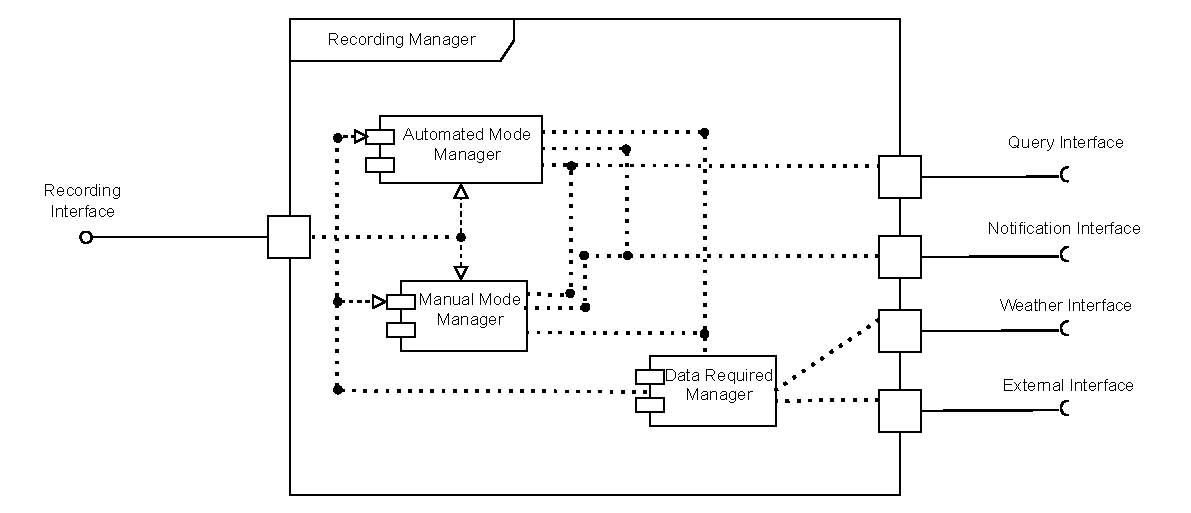
\includegraphics[width=\textwidth]{Images/Recording_Manager.drawio.pdf}
	\caption{Recording Manager}
\end{figure}

\begin{itemize}
	\item \textbf{Automated Mode Manager}: The Automated Mode Manager is responsible for the real-time acquisition of trip data without requiring constant user interaction.
	It implements the logic to infer cycling activity by monitoring the user's speed and initiates data collection when a specific threshold is exceeded. This component interfaces 
	directly with the mobile device's sensors to capture GPS coordinates for path reconstruction, as well as accelerometer and gyroscope readings to detect potential path irregularities. 
	\item \textbf{Manual Mode Manager}: The Manual Mode Manager handles the "offline reporting" workflow, allowing users to log cycling activities after they have occurred 
	It provides the functionality for users to reconstruct their route by inputting a sequence of street names or selecting segments on a map, rather than relying on real-time GPS tracking. 
	This component ensures that users can manually specify essential metadata, such as the total duration of the trip and the specific timeframes. Furthermore, it manages the annotation process, 
	allowing users to manually insert status updates or report obstacles for specific segments of the reconstructed path
	\item \textbf{Data Required Manager}: The Data Required Manager acts as an enrichment engine that enhances basic trip data with context and precise metrics using external services. 
	It interacts with the Weather Interface to retrieve historical meteorological conditions corresponding to the specific time and location of the recorded trip. 
	Additionally, it utilizes the External Interface to communicate with third-party mapping APIs for geocoding services and to calculate precise distances between coordinates, ensuring that the statistics displayed to the user, such as total distance covered and elevation gain, are accurate
\end{itemize}

\newpage
\section{Deployment View}
In this section of the document we focus on the deployment architecture of BBP and the motivations behind our design choices.

\begin{figure}[htbp]
	\centering
	\includegraphics[width=\textwidth]{2-deploymentView.pdf}
	\caption{Deployment View}
\end{figure}

We divided our system into three main tiers—presentation, application, and data tiers (better explained in Section~\ref{sec:three-tier})—to better isolate common features between all tangible and intangible instances of the objects involved. Below is a list of all actors and components in the system:

\begin{itemize}
	\item \textbf{Personal Device}: a personal device consists of a sensor device (here modeled as the union of all the device's movement sensors) and an operating system that can be either Android or iOS. It is intended as a personal piece of hardware such as a smartphone or smartwatch carried by the user throughout the execution of the application. The personal device communicates with the Application Server through a local instance of the application: every request made by the Application to the Application Server follows a RESTful interaction style over HTTPS.
	\item \textbf{API Gateway}: it is a node offered by a third party (such as AWS or Google Cloud Services) that provides a built-in Web Application Firewall (WAF) and a load balancer to distribute traffic among multiple Application Servers, thus avoiding single points of failure.
	\item \textbf{Application Server}: it is a device that contains the core logic of the application and connects all the drivers required for the application to operate. It communicates with external APIs using REST and interacts with multiple databases through a continuously managed connection pool.
	\item \textbf{Database}: we opted for multiple databases (one primary database and several read-only replicas) with a connection pool managed by the Application Server, ensuring that databases are protected by a limited number of open connections. This approach minimizes concurrency issues and prevents overload. The number of connections can be adjusted according to traffic patterns to achieve an optimal balance between hardware usage and system efficiency. Linux was chosen as the operating system due to its open-source nature, and MySQL for its robustness.
\end{itemize}

A closer look at some of the internal components of the system follows:

\begin{itemize}
	\item \textbf{Application Artifact}: the client-side application, primarily used as the presentation layer. It stores a signed JWT (JSON Web Token) used for authentication and is connected to all sensors required to detect movements in automated mode using cross-platform mobile frameworks.
	\item \textbf{BBP Server App}: the core model of the application. It contains the business logic and ensures that all operations are coherent with user requests by following the Model-View-Controller (MVC) pattern. It hosts all managers and connects them to the necessary drivers used to interface with external tools.
\end{itemize}

\section{Runtime View}

\section{Component Interfaces}

\section{Styles and Patterns}
\label{sec:three-tier}

BBP will be developed using the client-server paradigm integrated with a three-tier architecture and the Model-View-Controller pattern. The goal of this combined architecture is to achieve a clear separation of concerns among system components and improve control over each tier. The tiers involved are:

\begin{itemize}
	\item \textbf{Presentation Tier}: this tier serves as the view component of the application and contains software that interacts directly with the user's hardware (i.e., the personal device and its sensors). It represents the top-level tier and is designed to be mostly stateless, although some user information is stored through JWT tokens for authentication. Its main functionality is to display information and available actions to the user, as well as present outputs generated by the backend. The presentation tier does not contain core business logic, preventing users from modifying it locally to perform unauthorized actions and keeping the application lightweight in terms of memory usage. To ensure platform independence, Flutter was adopted to provide a unified abstraction layer for accessing sensor information across operating systems.
	
	\item \textbf{Application Tier}: this tier contains the core logic of the system and is composed of the Application Servers. It validates and executes user actions according to the current system state. Acting as a middle tier, it processes data received from the presentation tier and returns meaningful information to the user. Multiple Application Servers are deployed to enable scalability; with the use of an API Gateway equipped with a load balancer, requests can be routed consistently to specific servers using the JWT as an identifier. In case of server failure, users can be transparently rerouted to other servers, avoiding downtime.
	
	\item \textbf{Data Tier}: this tier represents the main repository of user and application data. It consists of a primary database and multiple secondary read-only replicas, all accessed through a connection pool that regulates the number of active connections. This architecture avoids data-tier downtime by allowing replica promotion in case of primary database failure, while preventing data inconsistency issues that may arise from having multiple writable databases.
\end{itemize}

In addition to the three tiers, a third-party API Gateway connects the presentation tier to the application tier. To satisfy scalability and security requirements, the API Gateway includes a \textbf{load balancer} to distribute incoming connections and a \textbf{Web Application Firewall} to protect against common attacks. AWS and Google Cloud Services are examples of providers offering such solutions.

The overall architecture follows a \textbf{client-server} interaction model in which most operations are event-driven. The client initiates the majority of transactions, except for server-generated notifications (e.g., automated mode activation). All client requests are validated by server-side logic, ensuring that communication errors and malicious behaviors are intercepted. Since communication is handled through \textbf{REST} over HTTPS, error messages can be clearly encoded and traced in both front-end and back-end scenarios.

The primary design pattern adopted is \textbf{Model-View-Controller}. The Model contains the logical components that manage and process application data, the View represents the graphical interface presented to the user through the client application, and the Controller handles user input and coordinates interactions between the Model and the View.

\section{Other Design Decisions}

\subsection{JWT}
JWT was chosen for authentication because, when combined with the load balancer deployed within the API Gateway, it enables secure login and registration while supporting scalability. Token expiration times (time-to-live) can be customized to allow either long-lived sessions or frequent re-authentication, providing flexibility in security policies.

\subsection{Avoidance of Single Points of Failure}
The use of an API Gateway, a homogeneous set of Application Servers, and load-balanced routing eliminates single points of failure. This design allows the system to scale horizontally by adding servers, thereby increasing robustness and the ability to handle higher request volumes.

\subsection{Microservices}
A microservices-based architecture was adopted to improve functional scalability. Each manager is implemented as an isolated service coordinated through notification and query mechanisms. This approach facilitates targeted testing, simplifies maintenance, and improves error identification and resolution.

\subsection{Cross-Platform Availability}
By using Flutter, a single codebase is maintained for the client-side application, improving code readability and maintainability through a shared operating system abstraction. This choice also enables BBP to reach a wider user base by supporting multiple platforms.